\subsubsection{本走行・実験走行で見つかった課題}
\paragraph{コストへのロボットの乗り上げにより動作不能になる問題}
むぎまるチームのリタイアの原因は、navigation2が経路生成をする際に参照する
コストマップにおいて、ロボットがコストに乗り上げてしまったことである。
この状況をRvizを用いて可視化した際の画像を図\label{fig:mugimaru_result}に示す。
図中のピンク色の範囲は走行不可能領域のコスト、
青色の範囲はロボットの内接円半径を考慮した際のコストを表している。
つまり、ロボットの中心が青色の範囲に侵入すると
ロボットが走行不可能領域にいると判断される。
図\label{fig:mugimaru_result}からロボットの中心は
青色の範囲に侵入していることが確認できる。
この状態になると、navigation2は目的地までの経路及び動作を生成しなくなる。
この状態になった後、ロボットはリカバリー動作を実行したが、
それも有効に働かずナビゲーションを中断してしまった。

この問題への対策として、走行可能領域に入るまで
安全に配慮しながら動き回るというリカバリー動作を実装することが
一つ挙げられる。
図からロボットの前方には走行可能領域があることが確認できる。
その場所まで3D LiDARにより周囲の安全を確認しながら移動可能であれば、
この問題が発生した場合にでもナビゲーションを続行できるようになると考える。
%\begin{figure}[h]
%  \centering
%  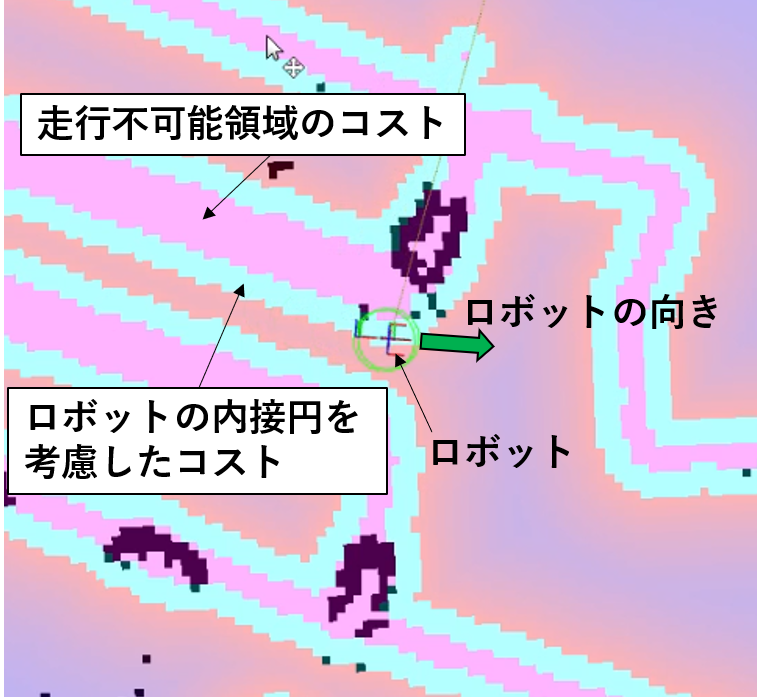
\includegraphics[width=1.0\linewidth]{figs/mugimaru_result.png}
%  \label{fig:mugimaru_result}
%  \caption{ロボットがコストマップに乗り上げた状況の図} 
%\end{figure}

\paragraph{前方のロボットへの追従}
実験走行の際に市役所裏の細い道で、前方で停止しているロボットを
無理に追い越そうとして、ロボットや周囲の障害物に衝突しそうになる
事例が見られた。
追い越そうとする際には、前方のロボットと障害物との間にできた
僅かな隙間を通るように経路を生成していた。
しかし、

% コストマップは、環境中の障害物情報やコースの情報を持ち、
% ロボットの障害物との衝突やコースアウトなどを防ぎながら
% ナビゲーションをするために用いられるデータである。


% ツナチームは、7/15、7/16、11/4、11/8、11/9の計5日間、実験走行および本走行に参加した。
% ike\_navは7月末から開発され、11/7に実機で使える状態になり、
% 動作確認ができたのは11/8、11/9のみであった。
% %そのため、直前ギリギリまで勧めていた作業としては、まずまずの結果といえる。
% 一方、記録は表1のように440[m]となり、ike\_navは、
% 実機に搭載する前から不具合の少ないソフトウェアであったと言える。
% 
% \subsubsection{本走行・実験走行で見つかった課題}
% \paragraph{障害物回避の不安定さ}
% 本走行時、ike\_navの障害物回避の機能にはバグが含まれていた。
% A*によって障害物回避をするようなパスを生成し、それを追従することで障害物回避としていた。
% このA*では、推定位置からゴールまでの最短経路を導出しつつ、障害物回避を行うために、
% 独自のヒューリスティック関数を実装した。
% これが、うまく実装できていれば良かったが、距離が遠いほど障害物回避を回避しようとしなくなるような
% 実装となっていた。そのため今後は,障害物回避の安定のために,このヒューリスティック関数の実装を見直し,修正をする予定である.

% \paragraph{尤度場、コストマップの作成に時間がかかる}
% ike\_navでは、尤度場とコストマップを自律走行を開始させる前に作成する処理がある。
% 地図としては、確認走行区間のみの情報しかないが、
% この処理に、1分ほどかかってしまっていた。
% これは、尤度場、コストマップの作成の実装に問題があるため、
% 作成部分の実装を見直し、修正をする予定である。
% @@@1分くらいいいんじゃない?@@@
